\section{Cryptographic Preliminaries}
% In this section, we define the notations used in this paper
% and explain the basic FHE primitives 
% forming the foundation for the architecture of \NAME. 
% In particular, we provide a systematic overview of 
% the vital homomorphic evaluations in \NAME.

% \subsection{Notation}
%In terms of FHE, we share similar notations to most previous works on LWE-based FHE. 
In this section, we summarize some of the important notations for FHE ciphertext
and FHE operators used throughout this work in \cref{pre:he_type},
and \cref{pre:he_circuits}, respectively.
For a complete list of notations, please refer to the appendix. 






% For LWE,
% $n$ can be any integer satisfying the security standard. For RLWE,
% $n$ is by default a power of 2, and the $2n$-th cyclotomic 
% polynomial $\Phi_{2n}(x)$ is used to instantiate the quotient ring $R_{n,q}$.
% We use the standard $B$-bounded discrete Gaussian distribution 
% $\chi$ to generate noises in \NAME. 




% \begin{table}[t!] 
% % \addtolength{\tabcolsep}{-2pt}
% % \footnotesize
%    \begin{center}
%    \vspace{-0em}
%        \caption{Summary of Notations}\label{tab: notations}
%        \vspace{-0em}
%      \begin{tabular}{c|l}
%         \toprule[1.0pt]
%         Notation & Description \\
%         \midrule
%         $\mathcal{D}$ & \\
%         $\mathcal{T}$ & \\
%         $\mathcal{Q} = (P_{1}, P_{2}, ...,P_{\lvert \mathcal{Q} \rvert}, G, \mathcal{F})$ & \\
%         $\mathcal{M}$ & \\
%         \midrule
%         $\mathbb{Z}_q$ & The ring of integers modulo $q$ \\
%         $\mathbb{Z}_{q}^{n}$ & The set of n-vectors over $\mathbb{Z}_q$ \\
%         $\mathbb{Z}[X]$ & The polynomial ring over $\mathbb{Z}$ \\
%         $\mathbb{Z}_{q}[X]$ & The polynomial ring over $\mathbb{Z}_q$ \\
%         $R_n$ & The cyclotomic ring   $\mathbb{Z}[X]/(X^n+1)$\\
%         $R_{n,q} $ & The cyclotomic ring $\mathbb{Z}_q[X]/(X^n+1) $ \\
%         $\chi$ & The noise distribution \\
%         $\Delta$ & The scaling factor \\
%         $\mathbf{a}$ & An element in vector domain \\
%         $\mathbf{a}[i]$ & The i-th component of $\mathbf{a}$ \\
%         $ \Tilde{a} $ & An element in polynomial ring \\
%         $ \Tilde{a}_i $ & The i-th coefficient of $\Tilde{a}$ \\
%         $ \hat{a} $ & The NTT-domain of element $a$ \\
%         $ {\rm LWE}(m) $ & An LWE ciphertexts encrypting $m$\\
%         $ {\rm RLWE}(.) $ & An RLWE ciphertexts  encrypting $m$\\
%         $ {\rm RGSW}(.) $ & An RGSW ciphertexts  encrypting $m$\\
%         \bottomrule[1.0pt]
%      \end{tabular}
%    \end{center}
%     \vspace{-0em}
% \end{table}

\subsection{Homomorphic Encryption}\label{pre:he_type}
For FHE notations, we use $\lambda$ to denote the security 
parameter and $p$ for the plaintext modulus. 
We use $q/Q/Q'$ to indicate different sizes of ciphertext modulus (generally $Q>q$),  
and $n/N/N'$ specify lattice dimensions (generally $N>n$).
$\mathbb{Z}_{q}$ refers to the set of integers 
modulo $q$. We define $R$ and $R_{Q}$ denote $\mathbb{Z}[X]/(X^{N}+1)$
and $\mathbb{Z}[X]/(X^{N}+1) \bmod Q$, respectively, for 
some ciphertext modulus $Q$ and polynomial degree $N$.
% In \cref{tab: notations},
% we list the commonly used notations throughout this work. 
Throughout this paper, we use bold lowercase letters (e.g., $\mathbf{a}$) for vectors, 
tilde lowercase letters (e.g., $\Tilde{a}$) for polynomials, 
and bold uppercase letters (e.g., $\mathbf{A}$) for matrices.

In this work, we mainly adopt the cryptographic constructions and 
techniques~\cite{DBLP:conf/ctrsa/hps19, DBLP:journals/access/s2cc2s, 
DBLP:journals/iacr/hs20,  DBLP:conf/asiacrypt/tfhepbs, 
pegasus,  DBLP:journals/tifs/apas,  cheetah,
ckksbootsparse, ckksbootstrap,ckksbootvariance} 
developed along both the CKKS~\cite{DBLP:conf/asiacrypt/CheonKKS17} and 
TFHE~\cite{DBLP:journals/joc/ChillottiGGI20} lanes of FHE schemes. Therefore, similar
to~\cite{heda}, we use ciphertexts that are based on both the 
learning with error (LWE) and ring learning with error (RLWE) hardness 
problems~\cite{regev2009lattices,lyubashevsky2010ideal}.
Moreover, we also make use of 
the ring variant of the GSW encryption scheme proposed in~\cite{DBLP:conf/crypto/GentrySW13}.
The concrete definitions are as follows.

$\bullet$ $\lwe_{\mathbf{s}}^{n, q}(m)$: The LWE ciphertext.
Here, we use a symmetric version of the LWE encryption function encrypting a single
integer message $m \in \mathbb{Z}_p$ under the secret key $\mathbf{s} \in 
\mathbb{Z}_{q}^{n}$ is given as: 
\[
    \lwe_{\mathbf{s}}^{n,q}(m) = (b, \mathbf{a}) = 
    (<-\mathbf{a}, \mathbf{s}> + \Delta m + e, \mathbf{a}).
\]
where $\mathbf{a} \in \mathbb{Z}_{q}^{n}$ is chosen uniformly at random, 
the noise $e$ is sampled from some distribution $\chi_{noise}$, and
$\Delta$ is a scaling factor to protect the least significant bits 
of the message from the noises. 

$\bullet$ $\rlwe_{\Tilde{s}}^{N,Q}(\Tilde{m})$: The RLWE ciphertext.
An RLWE ciphertext is defined as
\[
    \rlwe_{\Tilde{s}}^{N,Q}(\Tilde{m}) = (\Tilde{b}, \Tilde{a}) = (-\Tilde{a} \cdot \Tilde{s} + \Delta \Tilde{m} + \Tilde{e}, \Tilde{a}).
\]
for a vector of integer messages $\Tilde{m}\in R_{Q}$ under a secret key 
$\Tilde{s} \in R_{Q}$. Here, 
$\Tilde{a} \in R_{Q}$ is chosen uniformly at random and $\Delta$ is a scaling factor. 

$\bullet$ $\rgsw_{\Tilde{s}}^{N',Q'}(m)$: The RGSW ciphertext. First introduced in \cite{DBLP:conf/crypto/GentrySW13}, given a gadget vector $\mathbf{g} 
= (g_{1}, g_{2}, ..., g_{l}) \in \mathbb{Z}_{Q'}^{l}$, 
the RGSW encryption of a message $m 
\in \mathbb{Z}_p$ under the secret key $\mathbf{s} \in 
\mathbb{Z}_{q}^{n}$ is defined as: 
\[
    \rgsw_{\Tilde{s}}^{N',Q'}(m) 
    = \mathbf{Z} + m\mathbf{G} = (\mathbf{B}, \mathbf{A}) 
    \in \mathbb{Z}_{Q'}^{2l \times 2}.
\]
where $\mathbf{Z} \in \mathbb{Z}_{Q'}^{2l \times 2}$ contains $2l$ RLWE ciphertexts encrypting zeroes. 
$\mathbf{G}$ is defined as $\mathbf{G} = \mathbf{I}_{2} \otimes \mathbf{g}$,
where $\mathbf{I}_{2}$ is the identity matrix of size $n$ and 
$\otimes$ refers to the Kronecker product~\cite{kronecker} between two matrices.
Roughly speaking, an RGSW ciphertext is basically a collection of $2l$ RLWE ciphertexts.

We stress that all (R)LWE ciphertexts
contain certain levels of noise that can be amplified by the homomorphic
operators described below. Even if such noises may not cause decryption failures,
they contaminate the least significant bits of the plaintext messages and reduce 
the precision of the ciphertext until it becomes indecipherable.


% \subsection{Basic Homomorphic Circuits}
% We describe some homomorphic circuits that we use in this \NAME, 
% including arithmetic homomorphic circuits, logic homomorphic circuits 
% and the conversions between differents types of ciphertext.

\subsection{Homomorphic Operators} \label{pre:he_circuits}
% \NAME utilizes two fundamental types of circuits over FHE, 
% namely, arithmetic circuit which are basically made of additions 
% and multiplications,
% and logic circuit that consists of various logic gates (e.g., NAND, NOR).
Here, we explain the fundamental homomorphic operators used throughout this
work.
%including homomorphic arithmetic circuits, homomorphic logic circuits 
% as well as the conversion operators between different types of FHE 
% ciphertext.
Note that, we abbreviate the ciphertext notations to $\lwe(m)$, $\rlwe(m)$ 
and $\rgsw(m)$ when the parameters are not important to the discussion.

\subsubsection{Homomorphic Arithmetic Operators}
% As mentioned, homomorphic arithmetic circuits are circuits 
% purely based on the homomorphic addition and multiplication gates. 
% Using the well-known SV packing~\cite{DBLP:journals/dcc/SmartV14}
% technique, such gates operations can directly be translated to 
% additions and multiplications between polynomials.
We primarily use homomorphic arithmetic operators to evaluate
linear (i.e., polynomial) operations over RLWE ciphertexts.
Specifically, operations over homomorphic arithmetic circuits
are outlined as follows.

$\bullet$ $+$ , $-$ and $\cdot$: Ciphertext addition, subtraction
and multiplication. In this work, we consider an RLWE ciphertext
to be a tuple of polynomials, where 
additions ($+$) and multiplications ($\cdot$) are supported
between ciphertexts. For example,
given two RLWE ciphertexts $\rlwe_0= (\Tilde{b_0}, 
\Tilde{a_0}) $ and $\rlwe_1= (\Tilde{b_1}, \Tilde{a_1})$. 
The addition between the two ciphertexts is defined as 
$\rlwe(\ttm_0+\ttm_1)= \rlwe(\ttm_0)+ \rlwe(\ttm_1)= 
(\Tilde{b_0} + \Tilde{b_1} , \Tilde{a_0} + \Tilde{a_1})$.
Similarly, one can define the homomorphic subtraction 
between two RLWE ciphertexts. Finally,
given two RLWE ciphertexts $\rlwe(\ttm_0)$% = (\Tilde{b_0}, \Tilde{a_0}) $ 
and $\rlwe(\ttm_1)$ %= (\Tilde{b_1}, \Tilde{a_1})$ 
which encrypt plaintexts $\Tilde{m_0}$ and $\Tilde{m_1}$,
the homomorphic multiplication $\rlwe(\ttm_0)\cdot \rlwe(\ttm_1)$ results in 
$\rlwe (\ttm_0\cdot \ttm_1)$. More details on ciphertext multiplication
and the so-called relinearization process can be found 
in~\cite{DBLP:conf/crypto/brakerski12}.
% = (\Tilde{b_1} \cdot \Tilde{b_2} , 
% \Tilde{b_1} \cdot \Tilde{a_2} + \Tilde{b_2} \cdot \Tilde{a_1}, 
% \Tilde{a_1} \cdot \Tilde{a_2})$. 
% Subsequently, The process known as relinearization~\cite{DBLP:conf/crypto/brakerski12} 
% needs to be applied to $\rlwe_{\rm out}$, and the decryption of the relinearized
% ciphertext will produce $\Tilde{p_0} \cdot \Tilde{p_1}$.
% As the relinearization is not the optimization in this paper,
% we simply use \texttt{RLWEMul} denotes the multiplication with
% linearization process.

$\bullet$ $p(\rlwe(\ttm))$: Polynomial evaluation over the input ciphertext. 
For any polynomial $p(x)$, note that $p(\rlwe(\ttm))$ represents
the homomorphic evaluation of $p$ over the input
ciphertext $\rlwe(\ttm)$ encrypting $\ttm$, i.e., $\rlwe_{\rm out} = 
\rlwe(p(\ttm))= p(\rlwe(\ttm))$, 
decrypts to $p(\ttm)$. Here, the evaluation of $p$ can be realized by the 
homomorphic multiplication and addition operators. For example,
let $ct=\rlwe(\ttm)$, if $p(x)=x^3+x$, then $p(ct) = ct\cdot ct\cdot
ct+ct$. We note that there also exist more efficient algorithms
for evaluating $p$ over $\rlwe(m)$~\cite{ckksbootsparse, betterboot, 
improvedboot, ckksbootvariance}.

% $\bullet$ \textbf{Multiplication}: 

% $\bullet$ $\odot$: The external product operator.
% Let $\rgsw(\ttp)$ be an RGSW ciphertext, and let
% $\rlwe(\ttr)$ be an RLWE ciphertext.
% The external product $\rgsw(\ttp) \odot \rlwe(\ttr)$ results in an RLWE ciphertext 
% $\rlwe(\ttp\cdot\ttr)$ 
% %\mathbf{G}^{-1}(\Tilde{b}) \cdot \mathbf{B} + 
% %\mathbf{G}^{-1}(\Tilde{a}) \cdot \mathbf{A}$ 
% that encrypts $\Tilde{p} \cdot \Tilde{r}$,
% i.e., a ring-defined multiplication between the polynomials $\ttp$ and $\ttr$.
% Here, the $\mathbf{G}^{-1}$ is the gadget decomposition that satisfies 
% $<\mathbf{G}^{-1}(\Tilde{a}), \mathbf{g}> = \Tilde{a}$ for $\Tilde{a} \in R_{n,q}$.

% $\bullet$ $\odot$: The external product operator.
% Let $\rgsw(\ttp)= (\textbf{B}, \textbf{A})$ be an RGSW ciphertext
% which encrypts a plaintext polynomial $\Tilde{m}$, and let
% $\rlwe(\ttr) = (\Tilde{b}, \Tilde{a})$ be an RLWE ciphertext that encrypts $\Tilde{r}$.
% The external product $\rgsw(\ttp) \odot \rlwe(\ttr)$ results in an RLWE ciphertext 
% $\rlwe(\ttp\cdot\ttr) = \mathbf{G}^{-1}(\Tilde{b}) \cdot \mathbf{B} + 
% \mathbf{G}^{-1}(\Tilde{a}) \cdot \mathbf{A}$ that encrypts $\Tilde{p} \cdot \Tilde{r}$,
% i.e., a ring-defined multiplication between the polynomials $\ttp$ and $\ttr$.
% Here the $\mathbf{G}^{-1}$ is the gadget decomposition that satisfies 
% $<\mathbf{G}^{-1}(\Tilde{a}), \mathbf{g}> = \Tilde{a}$ for $\Tilde{a} \in R_{n,q}$.

% Although arithmetic circuits support efficient SIMD homomorphic operations, 
% they are limited by a fixed depth due to the noise growth in each function.
% In practice, they can only construct 
% queries with bounded filtering predicates.

\subsubsection{Homomorphic Logic Operators}
Different from homomorphic arithmetic operators,
% which can support efficient
% SIMD homomorphic operations, 
homomorphic logic  operators can be faster
when evaluating a deep chain of non-polynomial functions. The main
homomorphic logic operators are summarized as follows.
% , and
% are mainly based on single-instruction-single-data manner, and
% contains the following instructions:

$\bullet$ $\cmux(\rrgsw(\frakt), \rrlwe_{a}, \rrlwe_{b})$: 
The homomorphic selector. Note that the homomorphic selector works for
both $\rlwe$ and $\lwe$ ciphertext inputs, and we take the LWE case as an
example here.
Given $\lwe_a$ and $\lwe_b$
along with a control signal $\gsw(\mathfrak{t})$
that encrypts a binary 
plaintext $\frakt \in \{0,1\}$, 
$\cmux(\gsw(\frakt), \lwe_a, \lwe_b)$ homomorphically computes
\begin{align}\label{eq:cmux}
\frakt\text{ }?\text{ }\lwe_a\text{ }:\text{ }\lwe_b,
\end{align}
i.e., the function selects $\lwe_a$ if $\frakt=1$ and $\lwe_b$
if $\frakt=0$. 
%by evaluating $ \gsw \odot (\lwe_{a} - \lwe_{b}) + \lwe_{b}$.

% $\bullet$ $\br(\ttv, \lwe^{n, q}_{\bs}, \bBK)$: The homomorphic 
% blind rotate operator.
% $\br$ takes as input a polynomial $\ttv$ (i.e., the test vector 
% in~\cite{DBLP:journals/joc/ChillottiGGI20}),
% an LWE ciphertext $\lwe^{n, q}_{\bs}=(b, \ba)$ and a bootstrapping key
% $\bBK=(C_0, C_2, \cdots, C_{n-1})$, where $\bBK$
% %an RLWE ciphertexts $\rlwe = (\Tilde{b},  \Tilde{a})$ and $\ell + 1$ coefficients 
% is a collection of RGSW ciphertexts encrypting each of the
% elements in $\bs$, i.e., $s_0, s_1, ...,\bs_{n-1}$.
% $\br$ generates an RLWE ciphertext $\rlwe(X^{-\rho}\ttv)$,
% where $\rho = b + \sum_{i=1}^{\ell}s_i \cdot a_i$. 

$\bullet$ $\pbs(\lwe, \bBK, T(x))$: The programmable bootstrapping operator.
Given an LWE ciphertext $ct = {\rm LWE}_{\mathbf{s}}^{n,q}(\lfloor \Delta m \rceil)$ 
and a discrete function $T(x)$, and the bootstrapping key $\bBK$, $\pbs$ outputs
$\lwe_{\mathbf{s}}^{n,q}(T(\lfloor \Delta m \rceil))$ 
with a constant (i.e., input-independent) noise level.

$\bullet$ $\texttt{HomGate}(\lwe(m_0), \lwe(m_1), \texttt{OP})$: The homomorphic logic gate.
Given two LWE ciphertexts $\lwe(m_0)$ and $\lwe(m_1)$ along with a two-input
logic gate $\texttt{OP}$,
$\homgate(\lwe(m_0), \lwe(m_1), \texttt{OP})$ produces $\lwe(\texttt{OP}(m_0, m_1))$.
Note that, except for homomorphic NOT gate which is simply the negation of the input
LWE ciphertext, other gates including XOR, AND, OR, NAND, etc., are evaluated 
based on $\pbs$. As a result, $\homgate$ always outputs a ciphertext with
a constant level of noise and permits circuits of unbounded depths to be
evaluated over the homomorphic gates.



% We provide more details on \texttt{BlindRotate}, \texttt{PBS}
% and \texttt{HomGate} in \cref{Appendix:Details of logical circuits}.

\subsubsection{Homomorphic Format Conversion Operators}
Since homomorphic operators work on  different types of homomorphic ciphertexts,
homomorphic format conversion operators are required to convert between
different ciphertext formats, e.g., from an LWE ciphertext to an RLWE ciphertext.
Here, we briefly summarize the functionalities for each of the conversion
operators.
% Specifically, it contains the transformation mechanism between 
% an RLWE ciphertext and $N$ LWE ciphertexts.

$\bullet$ $\sei(\rlwe(\ttm))$: The conversion from one $\rlwe^{N, Q}_{\tts}$
ciphertext to a set of $N$ $\lwe^{n, q}_{\bs}$ ciphertexts.
% Given an RLWE ciphertext $\rlwe(\ttm)$,
%which encrypts $\Tilde{p} \in R_{n,q}$.
Similar to \cite{DBLP:journals/joc/ChillottiGGI20}, $\sei$ 
outputs $N$ LWE ciphertexts $\mathbf{ct} = (ct_0, ct_1, ...,ct_{N-1})$
where $ct_i$ encrypts the $i$-th plaintext coefficient of the message 
polynomial $\ttm$.

$\bullet$ $\repack(\lwe_{0}, \cdots, \lwe_{N-1})$:
The conversion from a set of $N$ $\lwe^{n, q}_{\bs}$ ciphertexts to one
$\rlwe^{N, Q}_{\tts}$ ciphertext, which is basically the inverse of $\sei$.
However, we note that existing methods for $\repack$ end up
with significantly reduced precision in the resulting $\rlwe$
ciphertext.
As later explained in \cref{block: LWEsPack}, due to the 
underlying cryptographic limitations, existing methods devised 
for $\repack$ cannot be directly
applied to a DB setting which requires a large number of
high-precision aggregation operations~\cite{pegasus,conversionhaochen}.
% Given $N$ LWE ciphertexts $ct_1, ct_2, ...,ct_N$ where 
% $c_i = \lwe^{n}(m_i)$. $\repack$ outputs 
% an RLWE ciphertext $ct = \rlwe^{N}(\ttm)$
% where 
% $\ttp_i = p_i$. 
% As mentioned in \cref{related:HE}, existing 
% methods (notably~\cite{pegasus} and~\cite{conversionhaochen})
% could not be applied to homomorphic databases nat\"ively.

%$\bullet$ \textbf{Circuit bootstrapping} \texttt{LWEToRGSW}:
$\bullet$ $\cb(\lwe, \bBK)$: The conversion from an $\lwe^{n, q}_{\bs}$ ciphertext
to an $\rgsw^{N', Q'}_{{\bf{\tts}}}$ ciphertext. $\cb$ is generally used to convert
a $\homgate$ result in the $\lwe$ format to an $\rgsw$ switching signal for the $\cmux$
operator. 
% More details of $\cb$ can be found 
% in~\cite{DBLP:journals/joc/ChillottiGGI20}.
%\textbf{Circuit bootstrapping} \texttt{LWEToRGSW}:

Due to space limitation, more details on $\br$, $\pbs$, $\homgate$,
$\sei$, $\repack$ and $\cb$ can be found in the related 
literature~\cite{DBLP:conf/asiacrypt/tfhepbs,conversionhaochen}.


%\subsection{homomorphic database} \label{pre: he_db}
%% here we introduce the definitions and notations related to database
%% and query processing.
%% 
%for db notations, we use $\db$ to denote the entire outsourced database containing
%$|\db|$ tables, where each table $\dbtab$ consists $\dbtabrowsize$ rows 
%and $\dbtabcolsize$ columns.
%% we define $\mathcal{d}$ denotes the database and the number of tables 
%% in $\mathcal{d}$ is $\lvert \mathcal{d} \rvert_{\mathcal{t}}$. 
%% for each table $\mathcal{t}$, it contains 
%% $\lvert \mathcal{t} \rvert_{r}$ rows and 
%% $\lvert \mathcal{t} \rvert_{c}$ columns.
%we represent $\mathcal{t} 
%= (t_1, t_2, ..., t_{\dbtabcolsize})$
%where $t_i$ is a vector of size $\dbtabrowsize$
%and refers to the i-th column of $\mathcal{t}$.
%we define the encrypted table 
%$\mathcal{ct} = 
%(ct_1, ct_2, ..., ct_{\lvert \mathcal{t} \rvert_{c}})$ 
%where $ct_i$ refers to the ciphertext of $t_i$.
%
%a query $\mathcal{q} = (p_{1}, p_{2}, ..., p_{\lvert \mathcal{q} \rvert_p}, {b}, {g})$
%implements the function of filtering and aggregation from
%a database table $\mathcal{t}$ and consists of the following parts:
%
%$\bullet$ $p_1, p_2, ...,p_{\lvert \mathcal{q} \rvert}$ are 
%$\lvert \mathcal{q} \rvert$ predicates,
%where each predicate $p_i$ is a tuple of $(\pop_i, \pattr_i, \val_i)$.
%here, $\pop_i$ is the exact comparison operator,
%$\pattr_i$ depicts the attribut,
%and $\val_i$ is the predicate value.
%taking \cref{fig: sql_example} as an example, here,
%the $\lvert \mathcal{q} \rvert$ is 3,
%$p_i(o)$ is \texttt{==},
%$p_i(a)$ is the attribute index of \texttt{id},
%and the $p_i$ is \texttt{2158}.
%
%$\bullet$ ${b} = (b_1, b_2, ...,b_{\lvert {b} \rvert})$
%are $\lvert {b} \rvert$ numbers logic gates between 
%different predicates.
%for instance,
%in \cref{fig: sql_example},
%the $\lvert {b} \rvert$ is 2 and
%both the $b_1$ as well as the $b_2$ are \texttt{and} gates.
%
%$\bullet$ ${g} = (g_1, g_2, ...,
%g_{\lvert {g} \rvert})$
%are $\lvert {g} \rvert$ numbers of aggregation field
%where each field $g_i$ includes 
%the aggregation function $g(f)_i$
%and the aggregation attribute index $g(a)_i$.
%as depicted in listing \ref{code:sql},
%the $g_1$ is \texttt{avg(hr)}, 
%the $g(f)_1$ is the \texttt{avg} function
%and the $g(a)_1$ is the attribute index of \texttt{hr}.
%note that, in queries like \texttt{select * from ...}, 
%the $\lvert {g} \rvert_g$ is equal to 
%$\lvert \mathcal{t} \rvert_{c}$
%and each aggregation function in $g_i$ is an identity function.
%
%\begin{figure}[t!]
%   \begin{center}
%   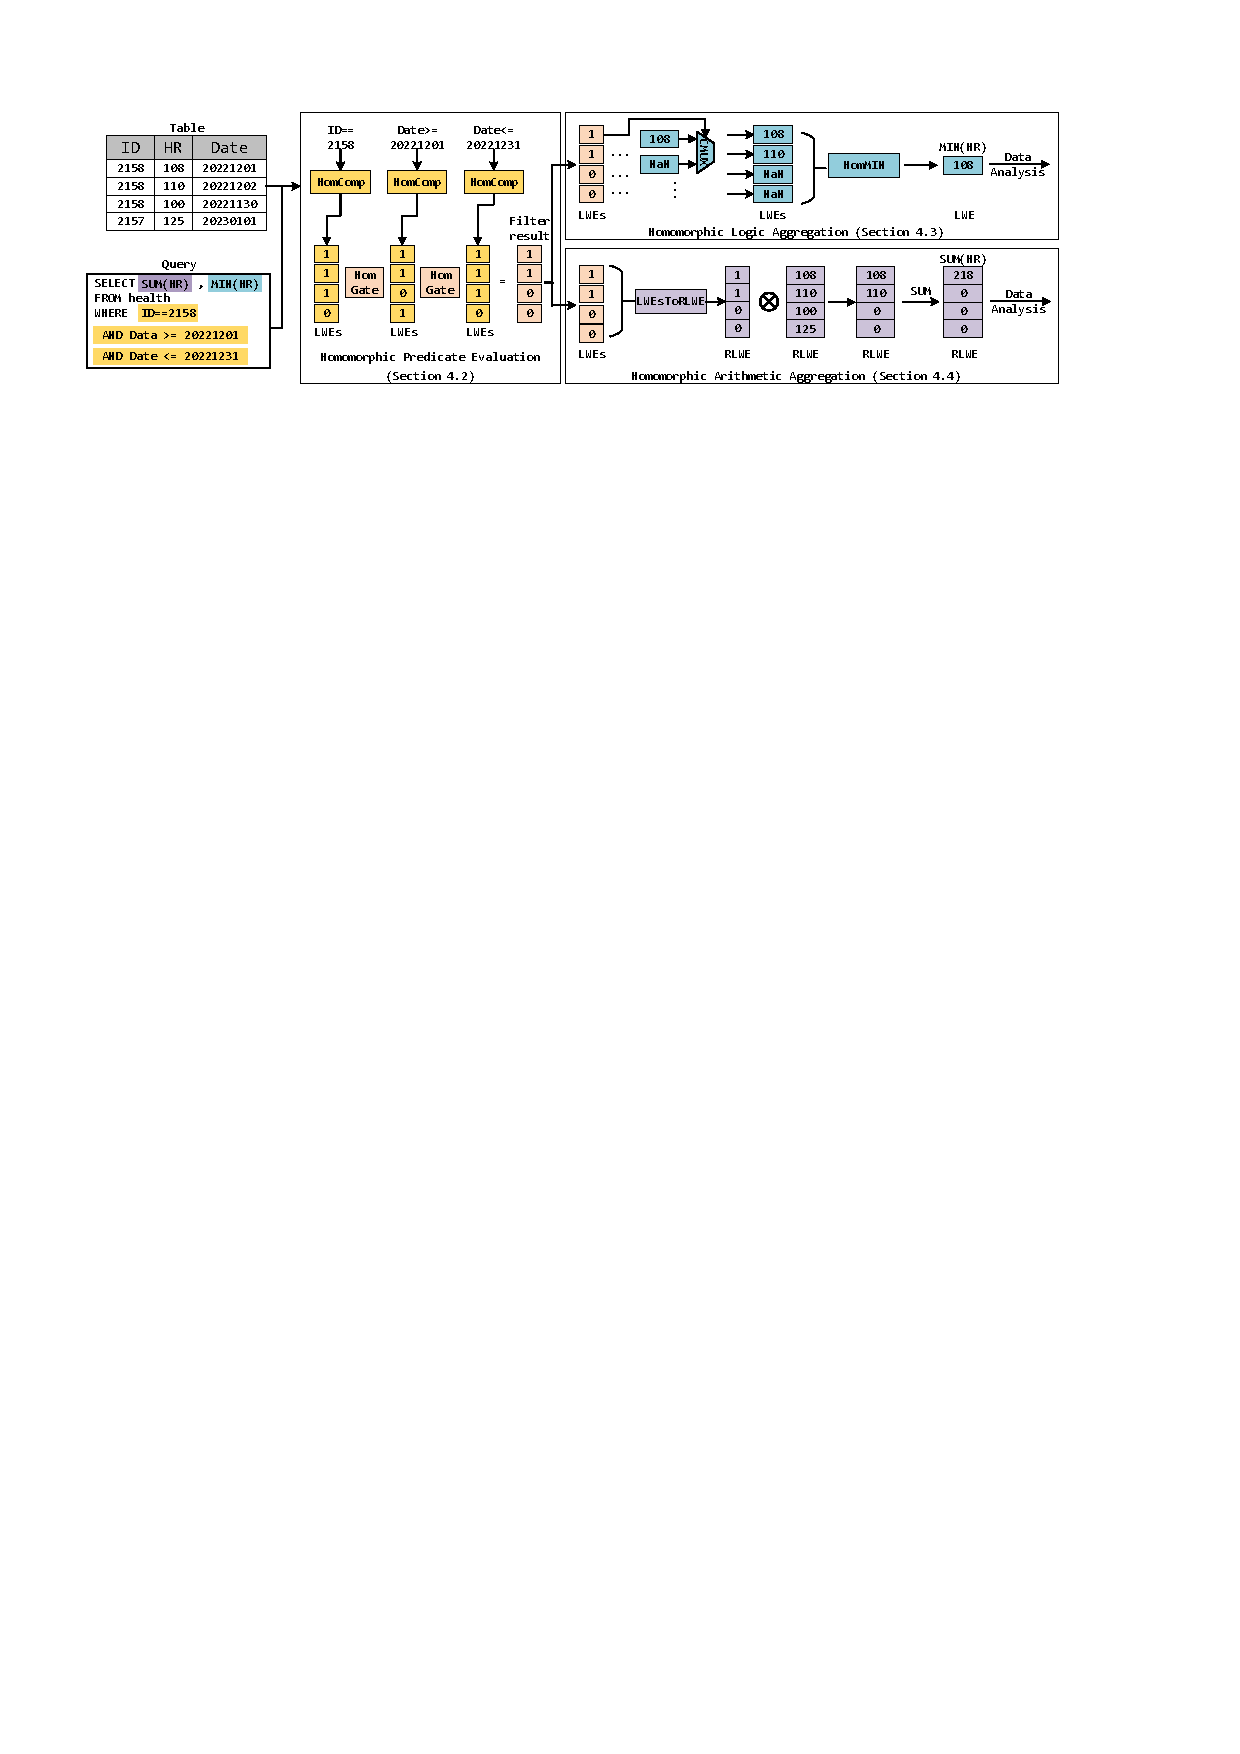
\includegraphics[width=\linewidth]{figure/query_evaluation.pdf}
%   \end{center}
%    \vspace{-0.5em}
%      \caption{sql query example.} 
%   \label{fig: sql_example}
%   \vspace{-0.5em}
%\end{figure}
%
%after the query processing, 
%the result is
%$\mathcal{r} = (r_1, ...,r_{\lvert g \rvert})$
%where $r_i$ is the aggregated value of $g_i$.
%in \cref{fig: sql_example}, $r = (r_1, r_2)$
%and $r_1$ is the value of \texttt{AVG(HR)}.
